\documentclass[11pt,english]{article} %% change font size here
\usepackage[T1]{fontenc}
%\usepackage[latin9]{inputenc}
\usepackage{caption}
\usepackage{datetime2} %% better DATE format
\usepackage{lipsum} %% for dummy text
\usepackage{graphicx}  %% for graphics

%%% VARS
\newcommand{\varTitle}{\ignorespaces
{{cookiecutter.title}}\ignorespaces}

\newcommand{\varName}{\ignorespaces
{{cookiecutter.author_first}} {{cookiecutter.author_last}}\ignorespaces}

\newcommand{\varAffiliation}{\ignorespaces
{{cookiecutter.author_institute}}, {{cookiecutter.author_uni}},
  {{cookiecutter.author_city}}, {{cookiecutter.author_country}}
}

%%%



%% here added for better citations
\usepackage[comma]{natbib} %% Here goes the natbib declaration
 %% NATBIB REF --> http://merkel.texture.rocks/Latex/natbib.php
 %% The \cite command functions as follows:
 %%   \cite{key} ==>                 Jones et al. (1990)
 %%   \cite[]{key} or \citep{key} => (Jones et al., 1990)
 %%   \cite[chap. 2]{key} =>         (Jones et al., 1990, chap. 2)
 %%   \cite[e.g.][]{key} =>          (e.g. Jones et al., 1990)
 %%   \cite[e.g.][p. 32]{key} =>     (e.g. Jones et al., p. 32)
 %%   \citeauthor{key}               Jones et al.
 %%   \citefullauthor{key}           Jones, Baker, and Smith
 %%   \citeyear{key}                 1990

%% use this natbib commands for numerical citations
%\usepackage[square,numbers]{natbib}

%% to include the references and remove contents in the table of content enable this:
\usepackage[nottoc,numbib]{tocbibind}
%% "notbib" Disables the inclusion of the Bibliography.
 %% "notindex" Disables the inclusion of the Index (inclusion of the Index of an
 %% "ltxdoc" class document is permanantly disabled).
 %% "nottoc" Disables the inclusion of the ToC.
 %% "notlot" Disables the inclusion of the List of Tables.
 %% "notlof" Disables the inclusion of the List of Figures.
 %% "chapter" Use chapter-level headings, if possible.
 %% "section" Use section-level headings, if possible.
 %% "numbib" Number the Bibliography heading (default is no number).
 %% "numindex" Number the Index heading (default is no number).
 %% "other" Use a non-traditional heading command. This option effectively requires
 %% the use of the \tocotherhead command.
 %% "none" Disables everything.

%% package for source code highlight
\usepackage{listings}

%% enable multi-language support
\usepackage{babel}

%% ==========================================================
%% SETUP DOCUMENT OPTIONS HERE
%% ==========================================================

%% ======================================
%% FONT
%% UNCOMMENT, to turn on sans serif font
%\usepackage{helvet}
%\renewcommand{\familydefault}{\sfdefault}
\usepackage{fontspec}
\setmainfont{Arial}


%%  icons
\usepackage{fontawesome}
%\usepackage{academicons}

%% ======================================
%% LINK COLORS
%% specify link colors here

%% Define own colors
%% allow html 
\usepackage[dvipsnames]{xcolor}
\definecolor{MyBlue}{HTML}{3c4f68}
\definecolor{light-gray}{gray}{0.95} %% good for source-code background

%% Colors that work well
%% xcolor: MidnightBlue, Sepia 
\usepackage[colorlinks=true, 
			urlcolor=MyBlue, 
			linkcolor=MyBlue,
			citecolor=MyBlue]{hyperref} 

%% ======================================
%% SECTIONS
%% UNCOMMENT, to turn off section numbering
%\setcounter{secnumdepth}{0}

%% UNCOMMENT, for centered section headings
%\usepackage[center]{titlesec}

%% ======================================
%% DOCUMENT MARGINS
%\usepackage{geometry}
%\geometry{verbose,tmargin=1.5cm,bmargin=2cm,lmargin=2cm,rmargin=2cm}
%% Alternative
\usepackage[a4paper,text={16cm,24cm},centering]{geometry}

%% ======================================
%% FOOTER and HEADER
\usepackage{lastpage}
\usepackage{fancyhdr}
\pagestyle{fancy}
\fancyhf{}%
\fancyhead[R]{
  \raisebox{-.7\baselineskip}[0pt][0pt]{\footnotesize\sf\varName{}}
}
\fancyhead[L]{\raisebox{-.7\baselineskip}[0pt][0pt]{\footnotesize\sf\varTitle{}}}
\fancyhead[C]{}
\fancyfoot[R]{\raisebox{.2\baselineskip}[0pt][0pt]{\footnotesize \sf \thepage\ / \pageref{LastPage}}}
\fancyfoot[L]{\raisebox{.2\baselineskip}[0pt][0pt]{\footnotesize \sf \Today}} %% \DTMDisplaydate{2016}{11}{01}{} for specific date
\fancyfoot[C]{}
% change to get lines on footer and header
\renewcommand{\headrulewidth}{0.25pt} %% set to 0pt to get rid of line
\renewcommand{\footrulewidth}{0.25pt}
%% color for line
\renewcommand{\headrule}{\hbox to\headwidth{\color{MyBlue}\leaders\hrule height \headrulewidth\hfill}}
\renewcommand{\footrule}{\hbox to\headwidth{\color{MyBlue}\leaders\hrule height \footrulewidth\hfill}}

%% make the plain style fancy too
\fancypagestyle{plain}{%
  \fancyhf{}%
  \renewcommand{\footrulewidth}{0.25pt}%
\fancyfoot[R]{\raisebox{.2\baselineskip}[0pt][0pt]{\footnotesize \sf \thepage\ / \pageref{LastPage}}}
\fancyfoot[L]{\raisebox{.2\baselineskip}[0pt][0pt]{\footnotesize \sf \Today}} %% \DTMDisplaydate{2016}{11}{01}{} for specific date
\fancyfoot[C]{}
  \renewcommand{\headrulewidth}{0mm}%
}   


%% UNCOMMENT, to remove page numbers 
%\pagenumbering{gobble}

%% ======================================
%% TITLE and authors
\title{\varTitle{}}
%% Affiliations in title
\usepackage{authblk}



\author[1,*]{\varName{}}
%\author[1,2]{Captn Awsome}
\affil[1]{\footnotesize\varAffiliation{}}
%\affil[2]{\footnotesize The second affiliation
%}
\affil[*]{\footnotesize corresponding author. email:
  \href{
    mailto:{{cookiecutter.author_email}}
  }{
    {{cookiecutter.author_email}} 
  } 
}
%% DATE in title
\date{\small \today } %% \DTMDisplaydate{2016}{11}{01}{}  for specifc date

%% ==========================================================

\usepackage{blindtext} %% for example text

%%%%%%%%%%%%%%%%%%%%%%%%%%%%%%%%%%%%%%%%%%%%%%%%%%%%%%%%%%%%%
%%% START 
\begin{document}

%% no paragraph indent at any paragraph
%\parindent 0pt 

\maketitle %% make title

%% Not used as we overwrite the plain style used for first page above.
%\thispagestyle{fancy} % for fancy footer on first page 

%% no number on current page
%\thispagestyle{empty}
%% all following pages no page number
%\pagestyle{empty}

%%%%%%%%%%%%%%%%%%%%%%%%%%%%%%%%%%%%%%%%%%%%%%%%%%%%%%%%%%%%%
%%% MAIN TEXT

%% include sections from other file
\begin{abstract}
Lorem ipsum dolor sit amet, consectetuer adipiscing elit. Ut purus elit, vestibulum ut, placerat ac, adipiscing vitae, felis. Curabitur dictum gravida mauris. Nam arcu libero, nonummy eget, consectetuer id, vulputate a, magna.
\end{abstract}


%\tableofcontents %% uncomment, to remove "Contents" section

\section*{Introduction}
\label{sec:introduction}

%% Include Fig1.png/.jpg here
\begin{figure}[t]
\captionsetup{font=footnotesize}
  \centering
    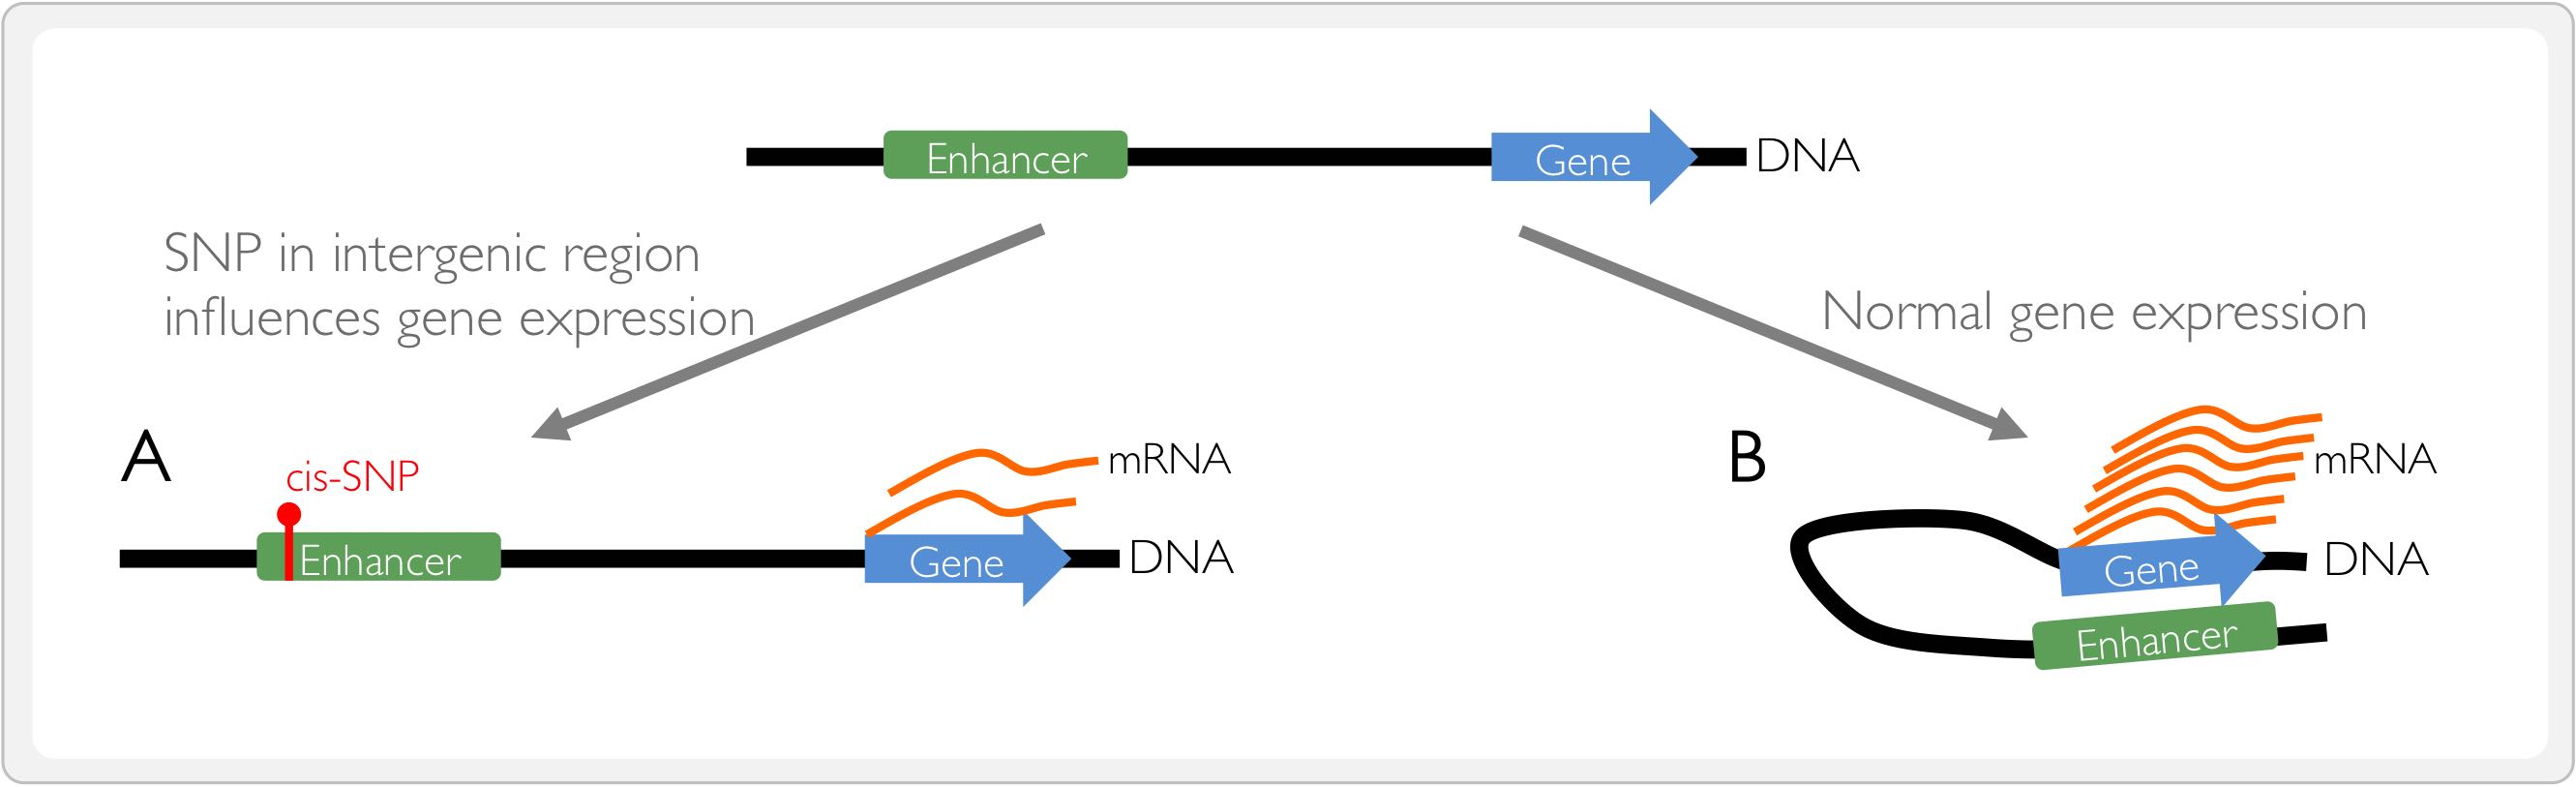
\includegraphics[width=\textwidth]{./images/Fig1} %% relative to main tex file
  \caption{The caption of the figure. \label{fig:fig1}}
\end{figure}

%% ref a figure 
\lipsum
Lorem ipsum dolor sit amet, consectetuer adipiscing elit (see Figure \ref{fig:fig1}).



\section*{Results}
\label{sec:results}

\noindent No indent in this paragraph \cite[see][]{Kim2010}! But we can use "citep" to get brackets like this \citep{Kim2010}!

\lipsum 

%% look up available icons here: http://mirror.aut.ac.nz/CTAN/fonts/fontawesome/doc/fontawesome.pdf
\faTwitter

%%  academicons not working yet.
%\aiGoogleScholar

%% code box ---------------------------
%% global listing settings
\lstset{frame=single,
  language=Python, 
  numbers=left, 
  backgroundcolor=\color{light-gray}, 
  basicstyle=\footnotesize }

\begin{lstlisting}
import sys, csv

# this is the main function
def main():
    return 'YAY'
\end{lstlisting}
%% code box ----------------------------
%% to include source code file:
%\lstinputlisting{source_filename.py}

\section*{Discussion}
\label{sec:discussion}

\lipsum

\section*{Conclusions}
\label{sec:conclusions}

\lipsum


\blinddocument %% example of article elements

%%%%%%%%%%%%%%%%%%%%%%%%%%%%%%%%%%%%%%%%%%%%%%%%%%%%%%%%%%%%%
%% Bibtex

{\footnotesize %% change to e.g. \small, etc.
%% needs bibstyle-apalike.bst -> Last FS, Last FS (2016) Title...
\bibliographystyle{./references/bibstyle-apalike}
%% natbib builtin style
%\bibliographystyle{humannat}

%% needs file library.bib -> global file in ~/Dropbox/configs/latex
%% which is the mendeley synced bibtex file
%\bibliography{\detokenize{~/Dropbox/configs/latex/library}} %% \detokenize allows the tilde
%% otherwise copy to local folder.
\bibliography{./references/library}
}

%%%%%%%%%%%%%%%%%%%%%%%%%%%%%%%%%%%%%%%%%%%%%%%%%%%%%%%%%%%%%
%%% END 
\end{document}
